\section{Hummingbird}

Hummingbird is the name of the base framework. In this section I'll explain how 
use the functionalities it features. The classes and methods that compose the framework 
are all contained inside the \textbf{hum} (\textbf{hum}mingbird) namespace.

For more information on each of the classes and methods check the hum namespace 
section of reference manual appended to this document.

\subsection{Game}

The Game class handles the game loop and the lifecycle of the game. To start
running a Game just call \texttt{run()} and the Game instance will enter the
following flow chart. The flow chart shows the lifecycle of a Game and the
different steps that happen through it.


\begin{figure}[H]
    \centering
    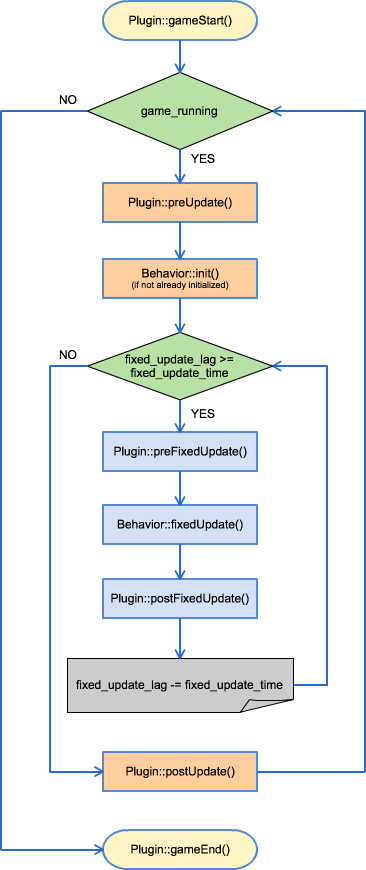
\includegraphics[width=0.5\textwidth]{game_loop}
    \caption{Game loop}
    \label{fig:game_loop}
\end{figure}

A Game instance can be queried for Time information at any step (when the
Game is running). This information can be the deltaTime(), which is the Time
that passed between the previous \texttt{update} and the current \texttt{update}; the fixedUpdateTime() which is
the Time that passes between \texttt{fixedUpdate} and \texttt{fixedUpdate} and is calculated
from the \texttt{fixed\_tickrate} constructor parameter; and the
fixedUpdateLag(), this last value is the Time since the last \texttt{fixedUpdate}.

The running state of the Game can be controlled by using setRunning(). If set
to \texttt{false} the game loop will exit and the Game will end. A Game instance
should not be reused once the Game is done running, as the final state is not
guaranteed in any way.

The Game class also owns the Actor object pool and therefore handles the
creation and destruction of Actors. Example code:

\begin{lstlisting}[caption=Creation and destruction of an Actor]
hum::Game game;
hum::Actor* new_actor = game.makeActor(); // creation of a new Actor;
// ...
game.destroy(new_actor); // mark the Actor to be destroyed.
\end{lstlisting}

Actors are not destroyed right away, but marked to be destroyed and destroyed
after \texttt{Plugin::postUpdate()}. All Actors are destroyed automatically after
\texttt{Plugin:gameEnd()}.

A Game instance can also contain Plugins. Plugins can implement functionality
for the Game such as a rendering pipeline, scene management, etc. They can be
added and queried by typename using addPlugin() and getPlugin() template methods
respectively (example below).

\begin{lstlisting}[caption=Plugin usage example]
class MyPlugin : public hum::Plugin {...};

hum::Game game;
MyPlugin* mp = game.addPlugin<MyPlugin>();

// somewhere else in the code (p.e. inside a Behavior)
MyPlugin* mp = game().getPlugin<MyPlugin>();
\end{lstlisting}

A Plugin shouldn't be added after calling run().

\subsection{Actor}

This class represents an object in the Game. You can create a new Actor by calling
Game::makeActor(). This method will create a new Actor and return it. The Game owns
the Actor and it controls its lifetime.

To destroy an Actor you must call Game::destroy(), not its destructor.
The Actor then, will be marked to be destroyed and after the next update step
it'll be deleted. Just before being deleted, the Actor will call its
Behaviors onDestroy() method.

An Actor, by default, doesn't have any behaviour and \textbf{you should not inherit
from it}.  Instead Actors are composed by Behaviors. These Behaviors are
the ones that must implement the behaviour of the Actor composed by them.

On the other hand, Actors do have a Transformation, accessible through transform()
and a reference to its Game, accessible through game().

A Actor can be \textbf{active} or \textbf{inactive}. If a Actor is \textbf{inactive} it exists,
all its Behaviors also exist and have been instantiated; but it \textbf{won't}
be updated. Same applies to its Behaviors.

Usage example. The Actor will be destroyed after 10 fixed updates:
\begin{lstlisting}[caption=Actor example]
// We define two Behaviors: A and B.
class B : public hum::Behavior
{
public:
    B(int x): value(x)
    {}

    int value;
}

class A : public hum::Behavior
{
public:
    A(int x): current(x)
    {}

    void init() override
    {
        last = actor().getBehavior<B>()->value;
    }

    void fixedUpdate() override
    {
        current++;
        if (current > last)
        {
            actor().game().destroy(actor());
        }
        hum::log("Count: ", current);
    }

private:
    int last, current;
}

int main()
{
    hum::Game g;
    hum::Actor* a = g.makeActor();
    // here we add the A and B to the Actor.
    A* t = a->addBehavior<A>(1);
    a->addBehavior<B>(10);
    g.run();
    return 0;
}
\end{lstlisting}


\subsection{Behavior}

Class from which inherit to implement and give an Actor behavior.

A Behavior always lives inside an Actor. Said actor takes care of the lifecycle
of the Behavior.

For creating a custom Behavior you may inherit from this class and override
the methods you need to implement the wanted functionality.

Behaviors must also implement a \texttt{static const char* behaviorName()} method that,
as the name hints, returns the class name. This is used for error reporting.

Usage example:
\begin{lstlisting}[caption=Behavior example.]
class PrintTransform : public hum::Behavior
{
public:
    void init() override
    {
        hum::log("Behavior initialized");
    }

    void fixedUpdate() override
    {
        hum::log("Actor transformation: ", actor().transform());
    }

    void onDestroy() override
    {
        hum::log("Actor destroyed");
    }

    static const char* behaviorName()
    {
        return "PrintTransform";
    }
}
\end{lstlisting}

\subsection{Transformation}

hum::Tranformation is a simple class that defines a spacial tranformation
of an object. That is it defines a 3D translation, rotation and scale, using
hum::Vector3.

The hum::Transformation class has a small and simple interface, its
position, rotation and scale members can be accessed directly
(there are no accessors like setPosition(), getPosition()) and it
contains no mathematical function other than the method transform(), which
accumulates transformations.

Usage example:
\begin{lstlisting}[caption=Tranformation example]
hum::Transformation t, t2;
t.position.x = 10.f;
t.rotation.z = 90.f;
t.scale.x = 0.5f;

t2.position.x = 5.f;
t2.rotation.z = -25.f;
t2.scale.x = 0.2f;

t = t.transform(t2);
hum::log(t); // hum::Transformation ( position=hum::Vector3( 15, 0, 0 ); rotation=hum::Vector3( 0, 0, 65 ); scale=hum::Vector3( 0.1, 1, 1 ) )
\end{lstlisting}

\subsection{Time and Clock}

The Time class represents a time interval. It has nanoseconds precision and can 
queried for its value in seconds, milliseconds, microseconds and nanoseconds.

The Clock class mesures time intervals and stores them in an instance of Time. 
Clock too has nanoseconds precision.

Usage example:
\begin{lstlisting}[caption=Clock and Time example]
hum::Clock clk;
while(game\_is\_running)
{
  hum::Time deltaTime = clk.reset();
  ... // Game code
}
\end{lstlisting}

\subsection{Logging}

The framework includes a set of methods to help the debug process by allowing to print 
messages depending on the environment (release or debug) and to various channels (standard 
or error).

\subsubsection{assert\_msg()}
Check a condition and if it fails, exit the program and print the message.

This method does nothing if NDEBUG is defined.

Usage example:
\begin{lstlisting}[caption= assert\_msg() example]
hum::assert\_msg(player\_x > 64, "Player is outside of the map! x=", player\_x);
\end{lstlisting}


\subsubsection{log()}
Print a message to the standard output.

T can be any type that has the operator \texttt{<<} overloaded.
It can also be any of the following classes:
\begin{itemize}
\item hum::Vector2
\item hum::Vector3
\item hum::Transformation
\item hum::Time
\item hum::Clock
\end{itemize}

Usage example:
\begin{lstlisting}[caption= log() example]
hum::log("Player position: ", actor().transform().position);
\end{lstlisting}

\subsubsection{log\_e()}
Print a message to the error output.

T can be any type that has the operator \texttt{<<} overloaded.
It can also be any of the following classes:
\begin{itemize}
\item hum::Vector2
\item hum::Vector3
\item hum::Transformation
\item hum::Time
\item hum::Clock
\end{itemize}

Usage example:
\begin{lstlisting}[caption= log\_e() example]
hum::log\_e("Player position: ", actor().transform().position);
\end{lstlisting}

\subsubsection{log\_d()}
Print a message to the standard output.

This method does nothing if NDEBUG is defined.

T can be any type that has the operator \texttt{<<} overloaded.
It can also be any of the following classes:
\begin{itemize}
\item hum::Vector2
\item hum::Vector3
\item hum::Transformation
\item hum::Time
\item hum::Clock
\end{itemize}

Usage example:
\begin{lstlisting}[caption=log\_d() example]
hum::log\_d("Player position: ", actor().transform().position);
\end{lstlisting}

\subsection{Plugin}
Class from which inherit to implement and give a Plugin for the Game.

A Plugin always lives inside the Game. The Game takes care of the lifecycle
of the Plugin.

For creating a custom Plugin you may inherit from this class and override
the methods you need to implement the wanted functionality.

For more information on the lifecycle of a Game see the Game class description.

Usage example:
\begin{lstlisting}[caption=Plugin example]
class DeltaTimePlugin : public hum::Plugin
{
  void gameStart() override {
    hum::log("Game just started");
  }

  void preUpdate() override {
    hum::log("delta time: ", game().deltaTime());
  }

  void preFixedUpdate() override {
    hum::log("fixed update lag: ", game().fixedUpdateLag());
  }

  void postFixedUpdate() override {
    hum::log("fixed update lag: ", game().fixedUpdateLag());
  }

  void postUpdate() override {
    hum::log("delta time: ", game().deltaTime());
  }

  void gameEnd() override {
    hum::log("Game just finished");
  }
}
\end{lstlisting}

\subsection{Kinematic}
Add Kinematic properties to the Actor. (Requires KinematicWorld).

This Behavior allows to give a velocity and an acceleration to an Actor. This way
the Actor's Transformation will change automatically overtime following a
kinematic movement.

Usage example:
\begin{lstlisting}[caption=Kinematic example]
hum::Game game;
game.addPlugin<hum::KinematicWorld>();

hum:Actor* actor = game.makeActor();
hum::Kinematic* k = actor->addBehavior<hum::Kinematic>();
k->velocity().position.x = 5;
k->acceleration().rotation.z = 2;
\end{lstlisting}

\subsection{KinematicWorld}
Plugin that handles the transformation (movement, scale or rotation)
of an Actor with a Kinematic behavior.


Usage example:
\begin{lstlisting}[caption=KinematicWorld example]
hum::Game game;
game.addPlugin<hum::KinematicWorld>();
\end{lstlisting}

\subsection{Exceptions}
\subsubsection{BehaviorNotFound}
Exception thrown when getting a Behavior from an Actor that
does not contain it. (see Actor::getBehavior())
\subsubsection{PluginNotFound}
Exception thrown when getting a Plugin from a Game that
does not contain it. (see Game::getPlugin())

\subsection{Vector2}
hum::Vector2 is a simple class that defines a mathematical
vector with two coordinates (x and y). It can be used to
represent anything that has two dimensions: a size, a point,
a velocity, etc.

The template parameter T is the type of the coordinates. It
can be any type that supports arithmetic operations (+, -, /, *)
and comparisons (==, !=), for example int or float.

You generally don't have to care about the templated form (hum::Vector2<T>),
the most common specializations have special \texttt{typedef}s:
\begin{itemize}
\item hum::Vector2<float> is hum::Vector2f
\item hum::Vector2<int> is hum::Vector2i
\end{itemize}

The hum::Vector2 class has a small and simple interface, its x and y members
can be accessed directly (there are no accessors like setX(), getX()) and it
contains no mathematical function like dot product, cross product, length, etc.

Usage example:
\begin{lstlisting}[caption=Vec2 example]
hum::Vector2f v1(16.5f, 24.f);
v1.x = 18.2f;
float y = v1.y;

hum::Vector2f v2 = v1 * 5.f;
hum::Vector2f v3;
v3 = v1 + v2;

bool different = (v2 != v3);
\end{lstlisting}

\subsection{Vector3}

hum::Vector3 is very similar to hum::Vector2, the only one difference is that it 
has three dimensions (x, y and z) instead of two. It works the same way Vector2 does 
and implements the same operations.

As for Vector2, you generally don't have to care about the templated form (hum::Vector3<T>),
the most common specializations have special typedefs:
\begin{itemize}
\item hum::Vector3<float> is hum::Vector3f
\item hum::Vector3<int> is hum::Vector3i
\end{itemize}

Usage example:
\begin{lstlisting}[caption=Vec3 example]
hum::Vector3f v1(16.5f, 24.f, 13.f);
v1.x = 18.2f;
float y = v1.y;

hum::Vector3f v2 = v1 * 5.f;
hum::Vector3f v3;
v3 = v1 + v2;

bool different = (v2 != v3);
\end{lstlisting}

\subsection{ResourceManager}
Class that implements the generic functionality of a resource manager.

This template class has three type parameters, two of which are optional. The
first is the type of the data to manage. The second one is the type of the
key to identify the managed data (\texttt{std::string} by default). The third is the data needed to load the
resource (\texttt{std::string} by default).

Usage example (manager for sf::Texture):
\begin{lstlisting}[caption=ResourceManager example]
class TextureManager : public ResourceManager<sf::Texture>
{
protected:
  sf::Texture* loadResource(const std::string& name) override
  {
    sf::Texture* resource = new sf::Texture();
    if (not resource->loadFromFile(name))
      return nullptr;
    return resource;
  }
};

//...

TextureManager tm;

if (!tm.load("cat", "cat.jpg")) {
  hum::log_e("Error loading cat.jpg");
}
if (!tm.load("dog", "dog.jpg")) {
  hum::log_e("Error loading dog.jpg");
}

sf::Texture* cat = tm.get("cat"); // get the texture

tm.free("cat"); // unload the cat texture manually

// when destroyed the resource manager will free all loaded resources.

\end{lstlisting}

